\chapter{Conclusion and Outlook} \label{ch:cando}

\section{8 TeV Inclusive Jet Results from CMS and ATLAS}

CMS\cite{CMS:2013kda} and ATLAS\cite{Aaboud:2017dvo} both reported the double differential cross section for inclusive jets at 8 TeV.  

\begin{figure}[h]
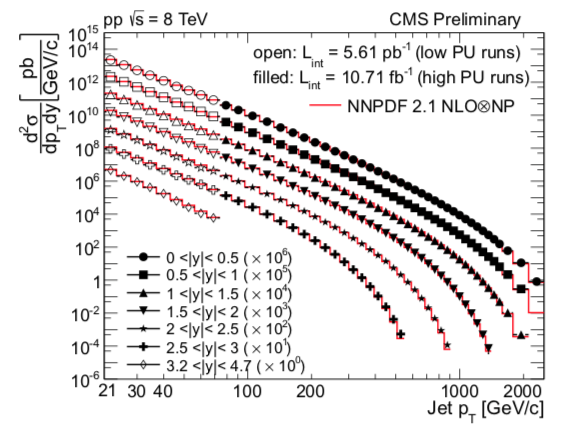
\includegraphics[width=10.0cm]{CMS8TeVJet}
\centering
\caption{8 TeV CMS inclusive jet cross sections with radii of R = 0.7 and binned by jet rapidity compared to NLO calculations with non-pertubative corrections\cite{CMS:2013kda}.}
\label{fig:CMS8TeVRescale}
\end{figure}

\begin{figure}[h]
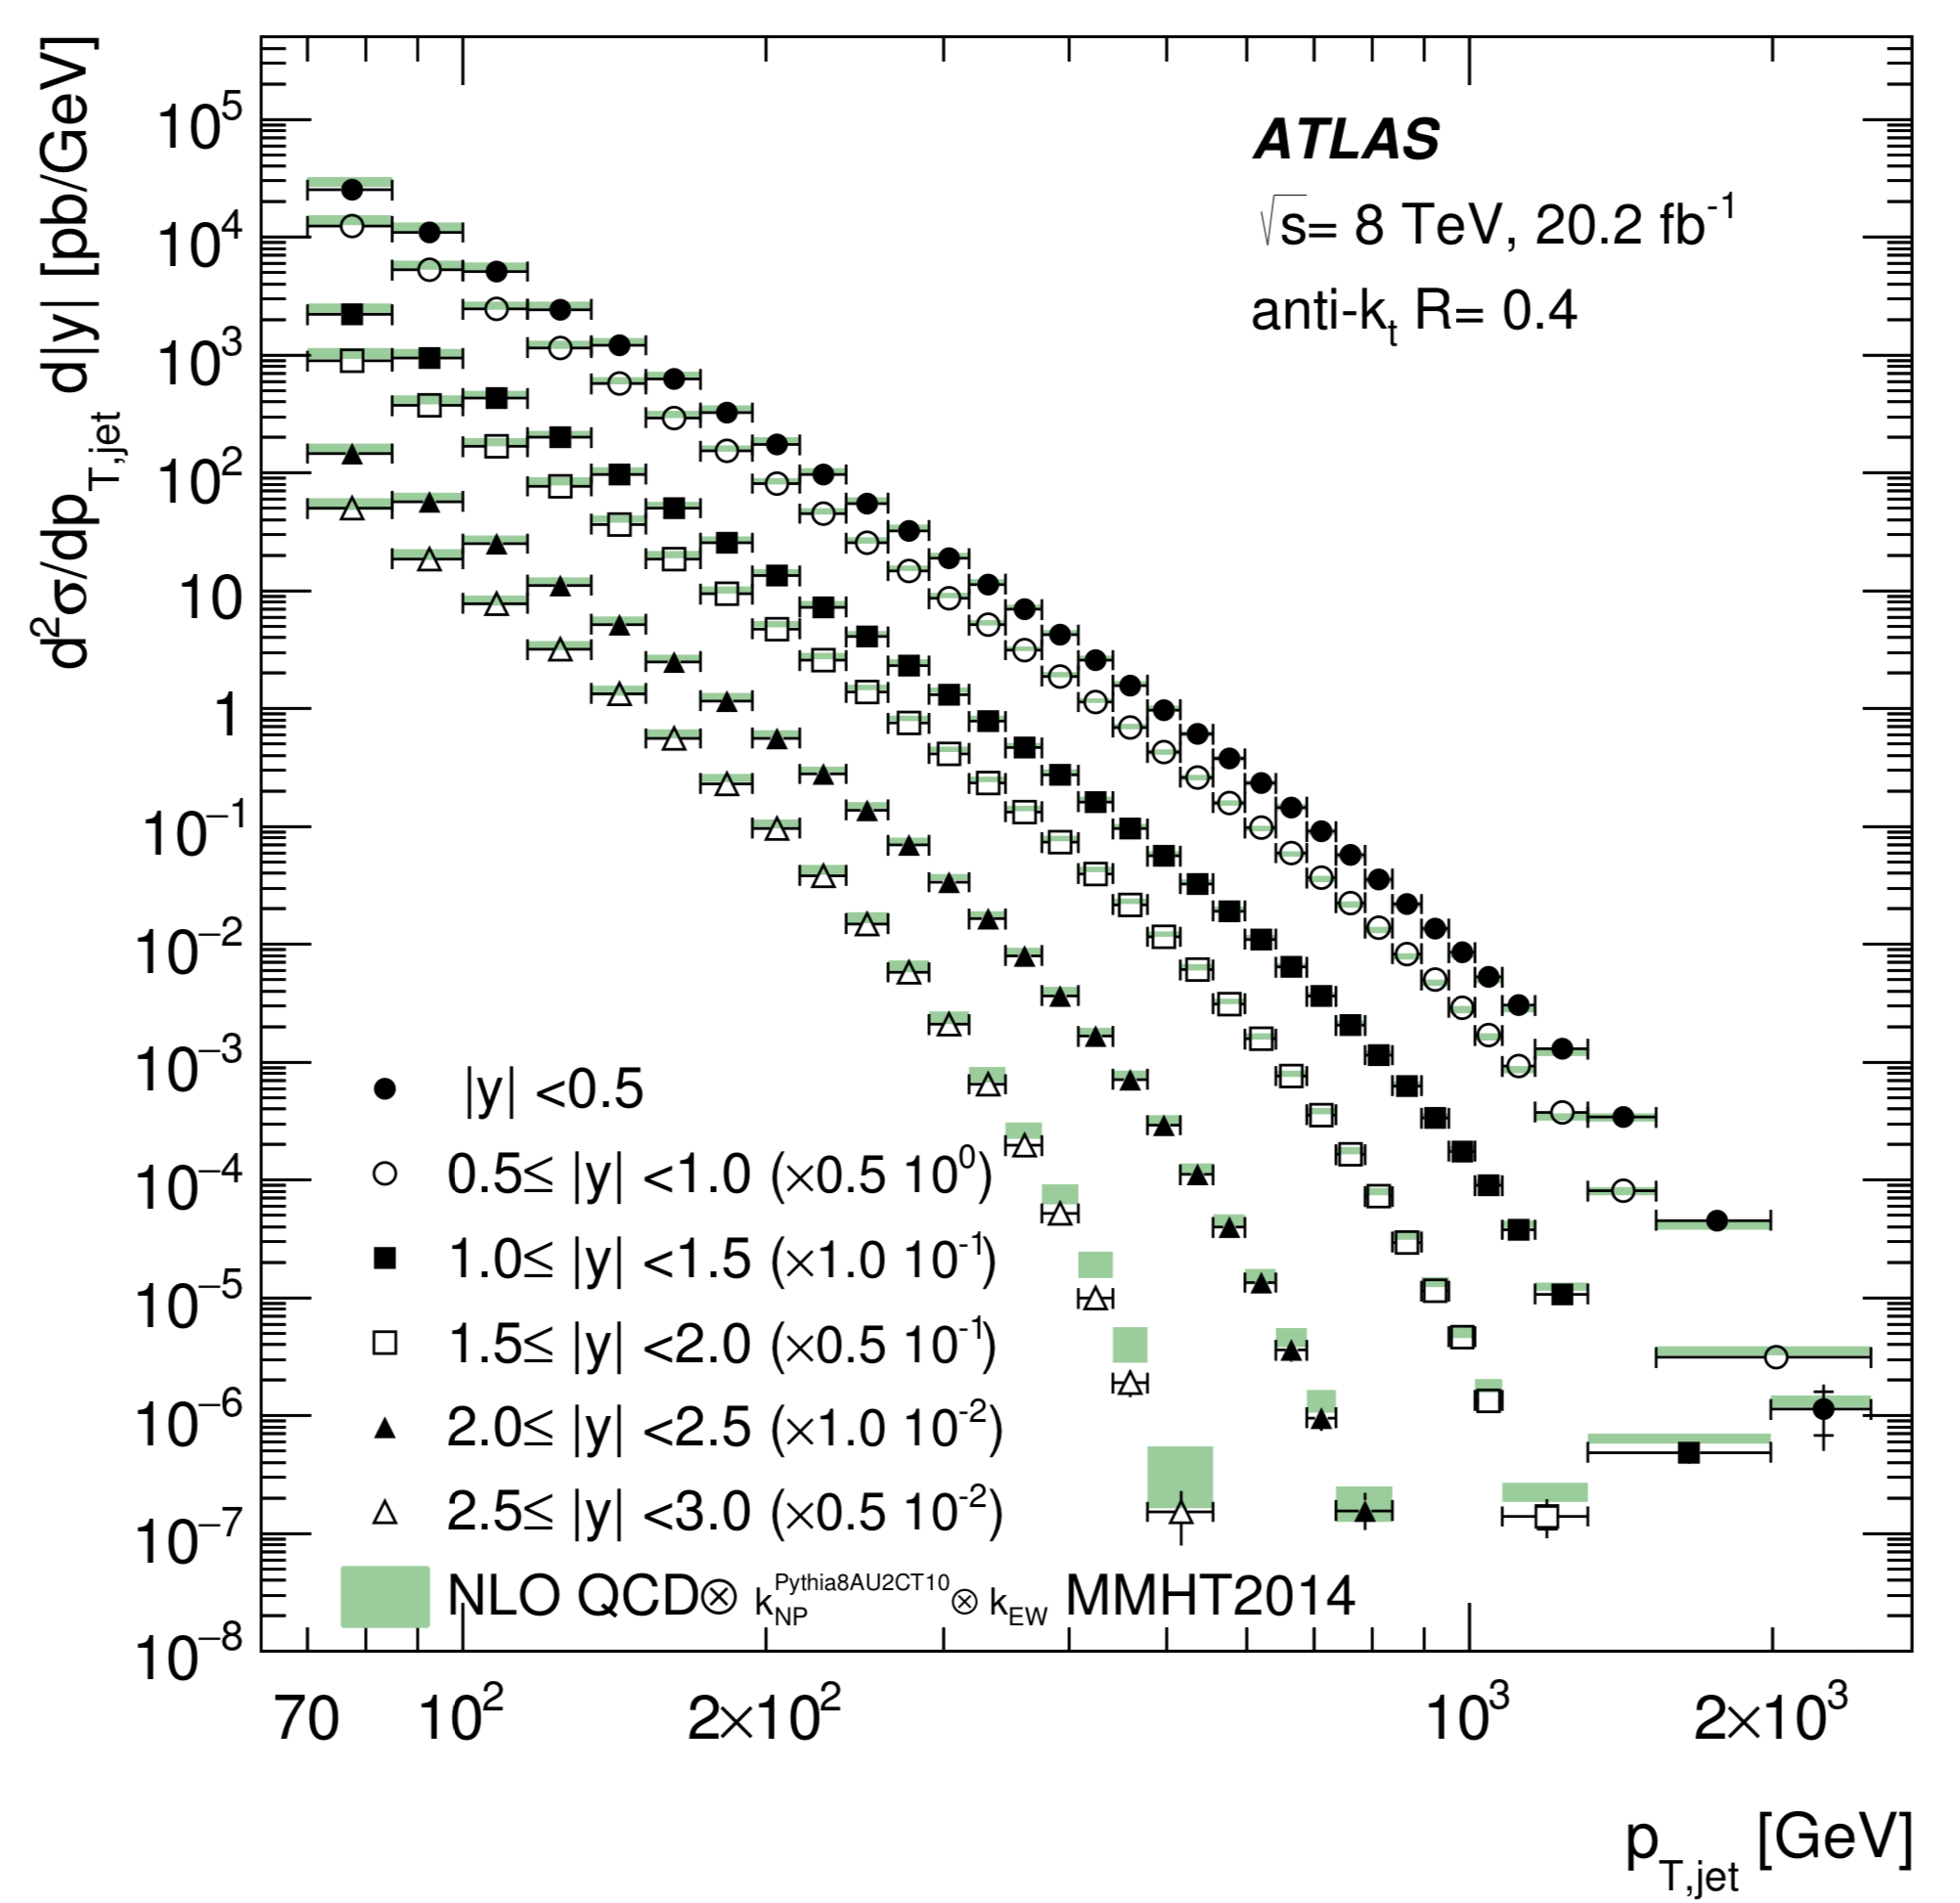
\includegraphics[width=10.0cm]{ATLAS8TeVJet}
\centering
\caption{R = 0.4 inclusive jet cross section at 8 TeV from ATLAS in binned by jet rapidity compared to NLO QCD predictions\cite{Aaboud:2017dvo}.}
\label{fig:ATLAS8TeV}
\end{figure}

\begin{figure}[h]
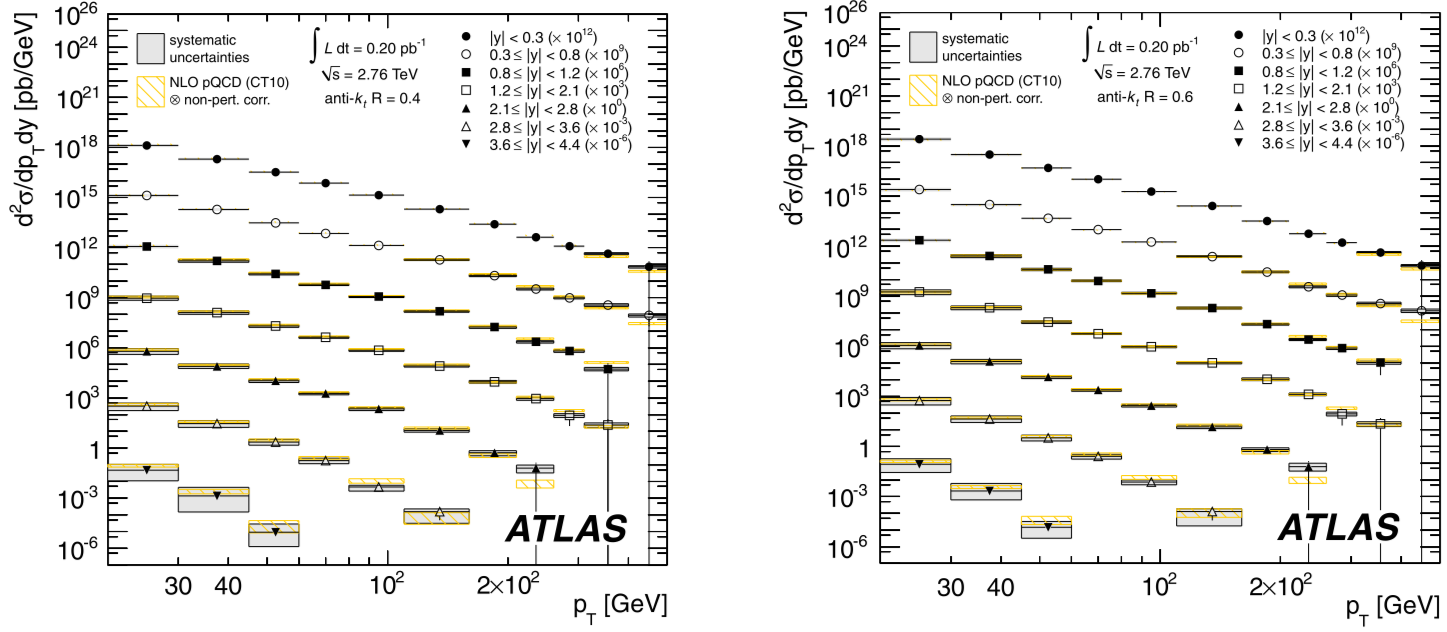
\includegraphics[width=14.0cm]{ATLAS8TeVJetRecaled}
\centering
\caption{The 8 TeV ATLAS jet cross sections rescaled to better show comparissons with NLO and non-pertubative calculations at low $p_{T}$\cite{Aaboud:2017dvo}.}
\label{fig:ATLAS8TeVRescale}
\end{figure}

\section{Inclusive Jet Spectra and Cross Section Ratios at 2.76 TeV}
Inclusive jet spectra and cross section ratios were measured in the ALICE experiment using a 2011 pp 2.76 TeV data sample\cite{MA2013319}.  Jets were reconstructed using TPC tracks and EMCal clusters with the FastJet Anti-$K_{T}$ algorithm.  Tracks with a minimum $p_{T} \geq \,$ 150 MeV and constrained to within 10 cm of the primary vertex were accepted into the jet finder.  EMCal clusters were 

\begin{figure}[h]
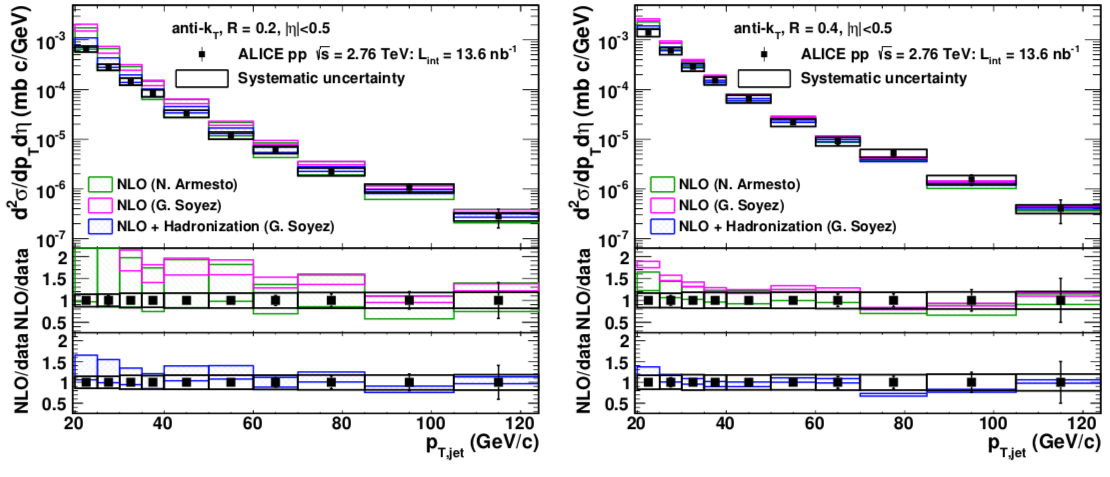
\includegraphics[width=17cm]{AliceppRongRong}
\centering
\caption{Inclusive differential cross section from the 2.76 TeV proton proton run with ALICE}
\label{fig:RunEff}
\end{figure}

\begin{figure}[h]
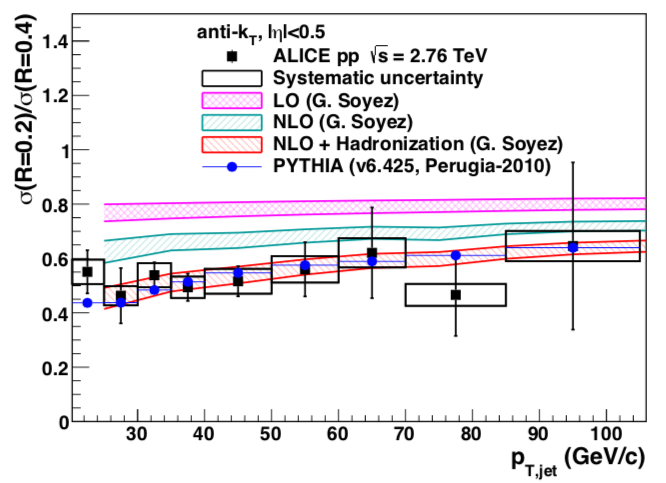
\includegraphics[width=10cm]{AliceRatioRongRong}
\centering
\caption{LHC state during the 8 TeV run. }
\label{fig:RunEff}
\end{figure}

\begin{figure}[!tbp]
  \centering
  \begin{minipage}[b]{0.49\textwidth}
    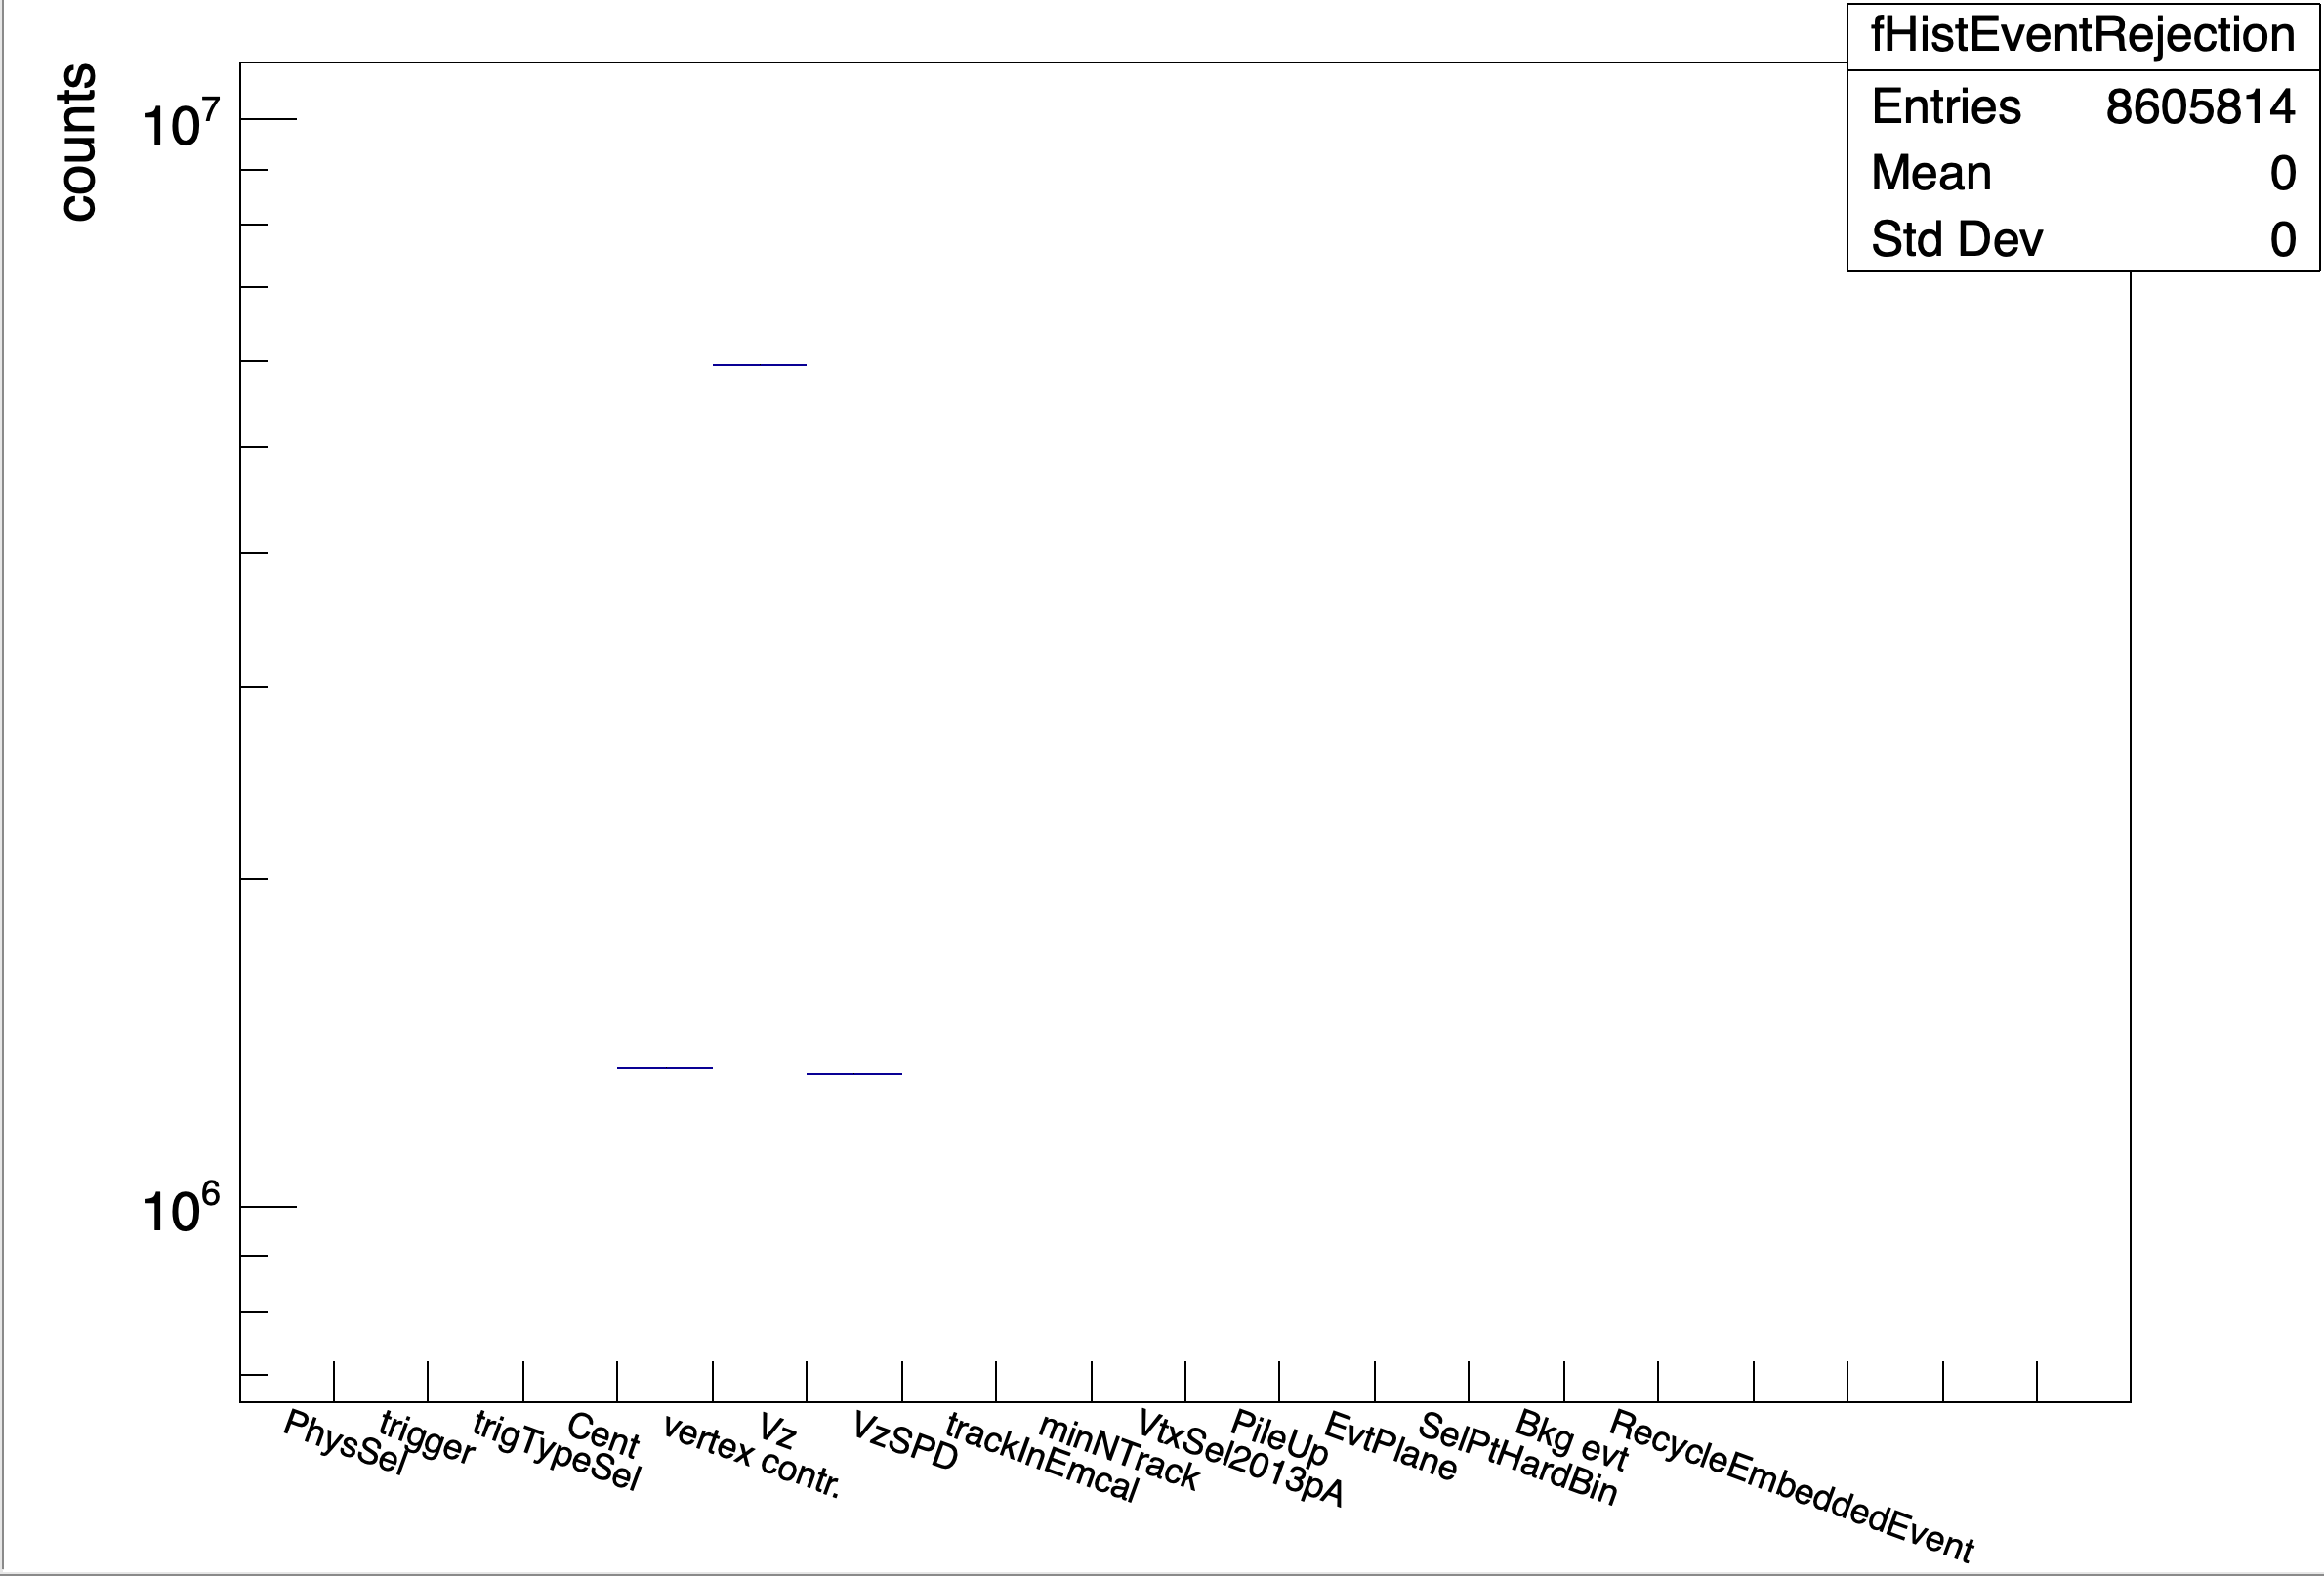
\includegraphics[width=\textwidth]{EventRejectionMB}
    \caption{Mimimmum Bias Event Rejection}
  \end{minipage}
  \hfill
  \begin{minipage}[b]{0.49\textwidth}
    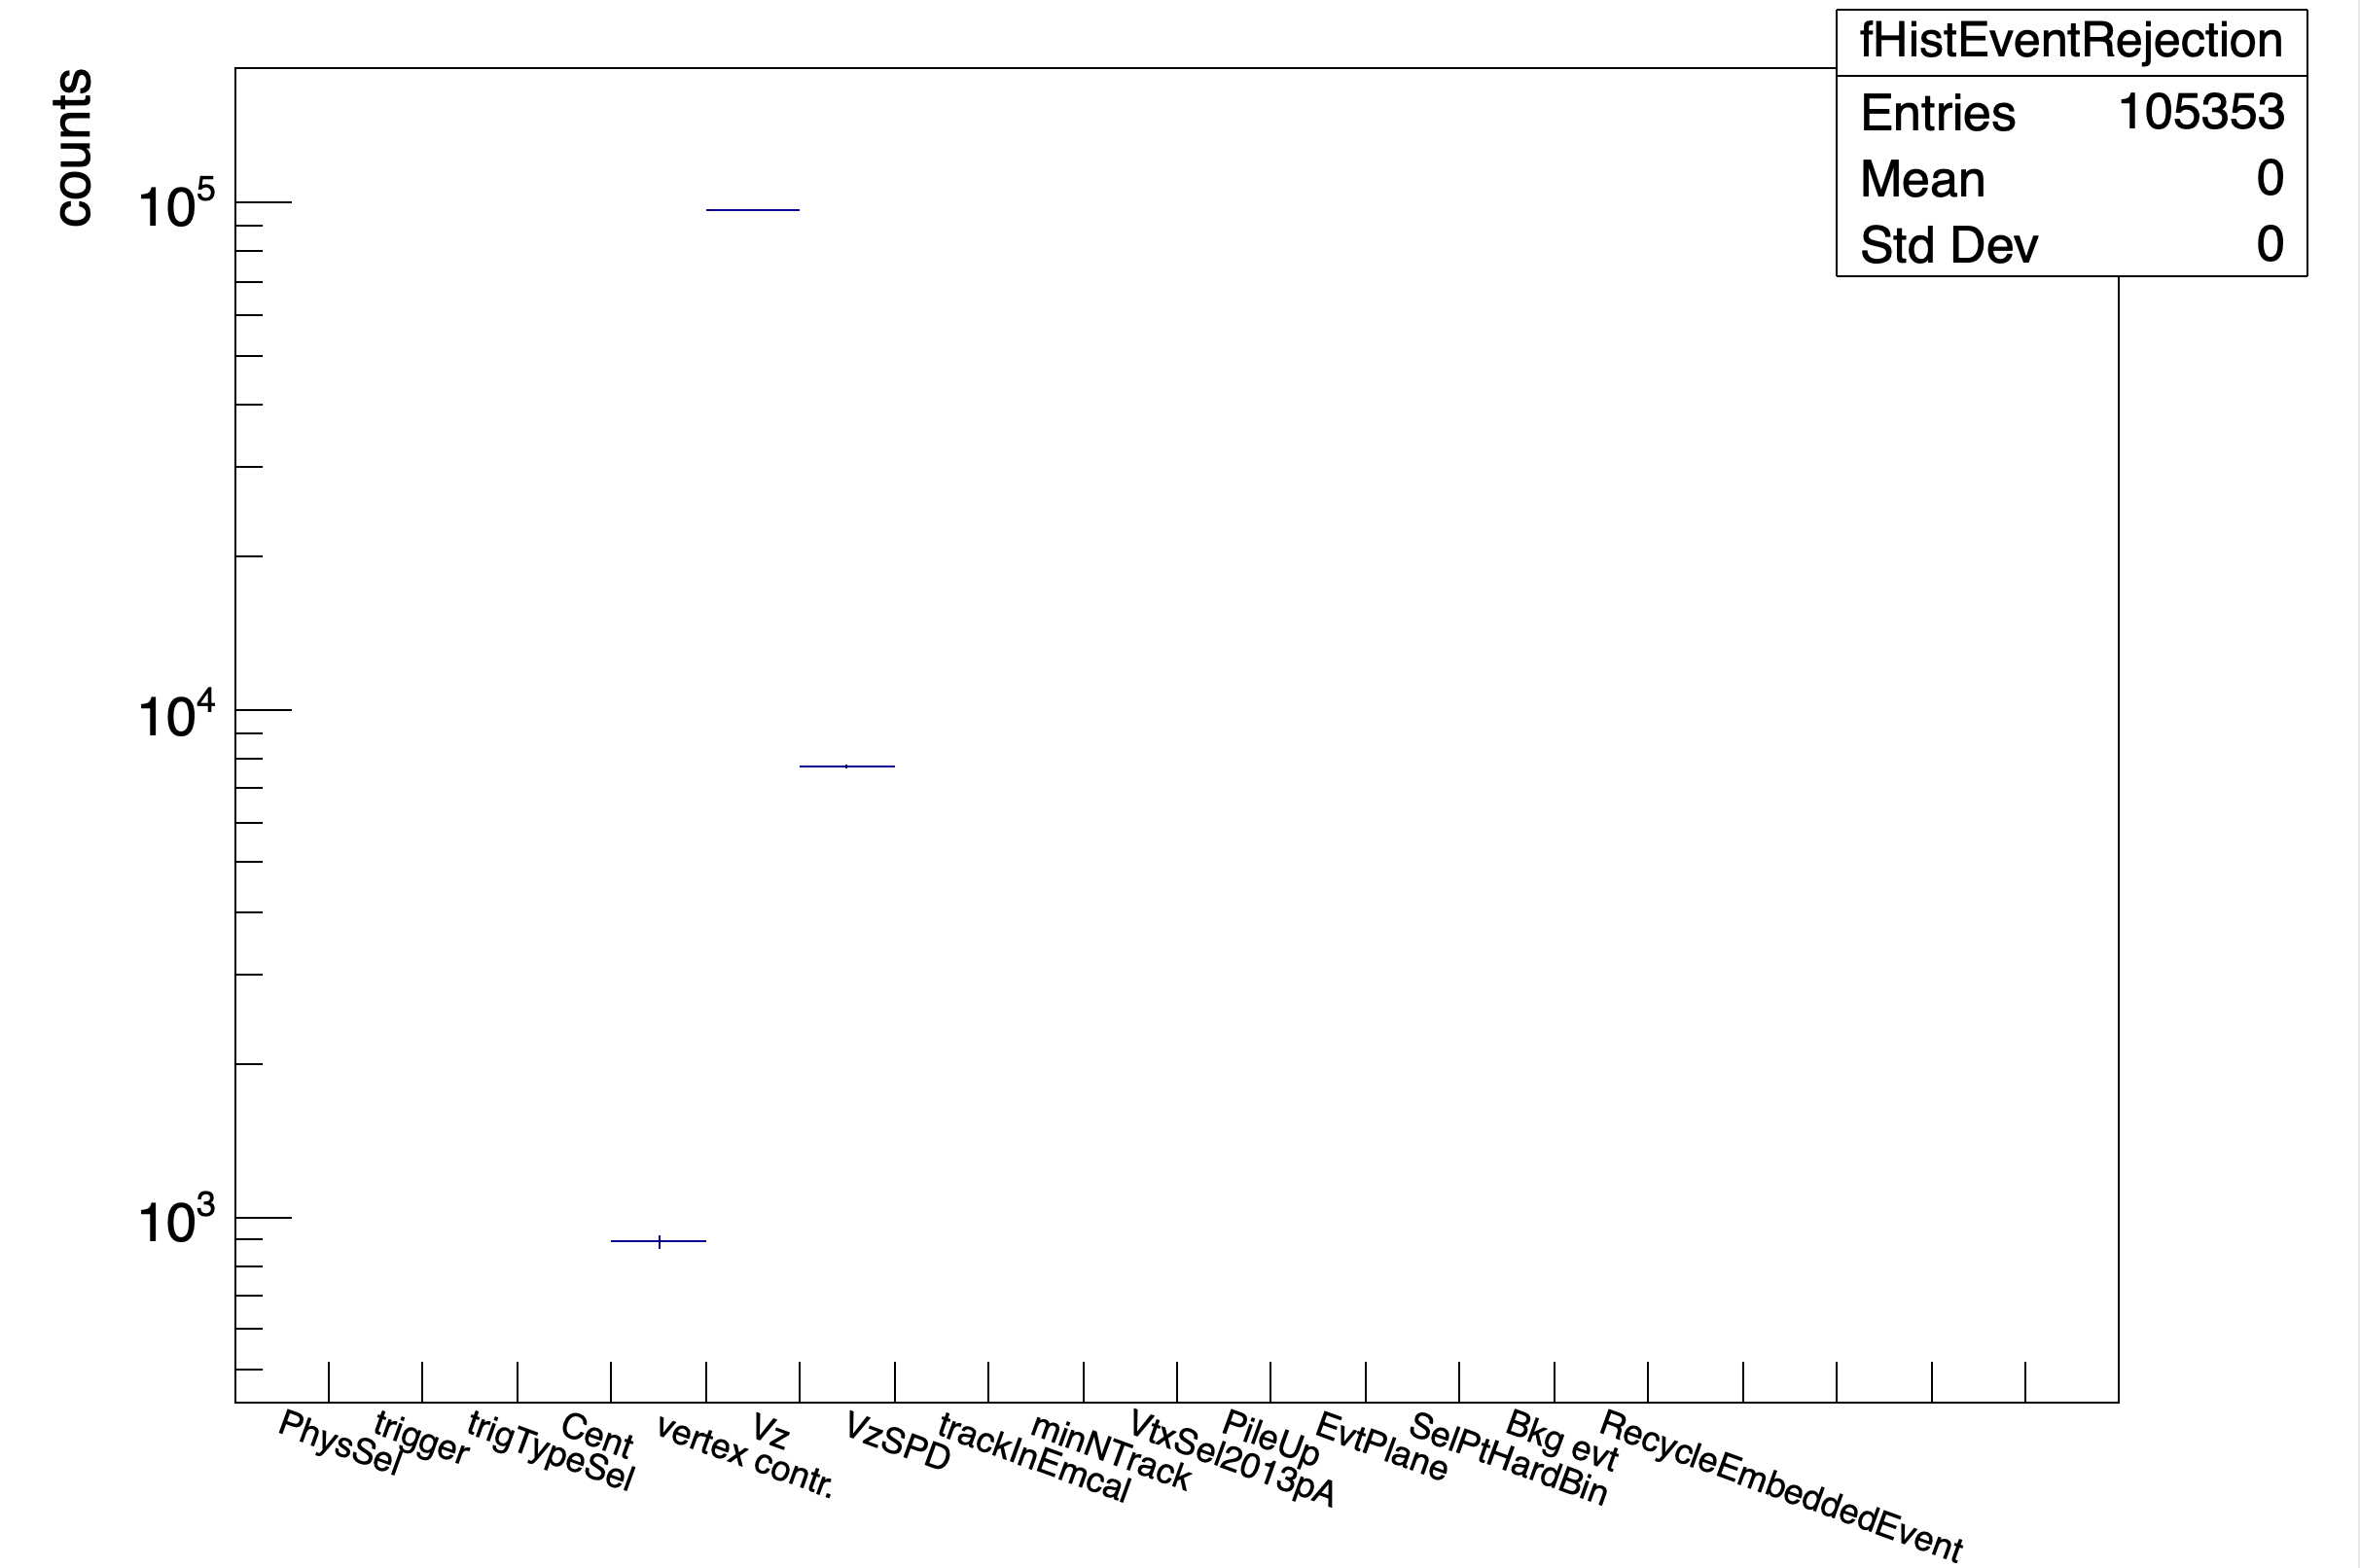
\includegraphics[width=\textwidth]{EventRejectionEGA}
    \caption{Emcal Triggered Event Rejection}
  \end{minipage}
\end{figure}